% Author: Izaak Neutelings (November 2020)
\documentclass[border=3pt,tikz]{standalone}
\usepackage{physics}
\usepackage{tikz}
\usepackage[outline]{contour} % glow around text
\usetikzlibrary{patterns,decorations.pathmorphing}
\usetikzlibrary{decorations.markings}
\usetikzlibrary{arrows.meta}
\usetikzlibrary{calc}
\tikzset{>=latex}
\contourlength{1.1pt}

\colorlet{mydarkblue}{blue!40!black}
\colorlet{myblue}{blue!70!black}
\colorlet{myred}{red!65!black}
\colorlet{myorange}{orange!90!black!90}
\colorlet{vcol}{green!45!black}
\colorlet{watercol}{blue!80!cyan!10!white}
\colorlet{darkwatercol}{blue!80!cyan!80!black!30!white}
\colorlet{metalcol}{blue!25!black!30!white}
\tikzstyle{piston}=[blue!50!black,top color=blue!30,bottom color=blue!50,middle color=blue!20,shading angle=0]
\tikzstyle{water}=[draw=mydarkblue,rounded corners=0.1,top color=watercol!90,bottom color=watercol!90!black,middle color=watercol!50,shading angle=20]
\tikzstyle{horizontal water}=[water,top color=watercol!90!black!90,bottom color=watercol!90!black!90,middle color=watercol!80,shading angle=0]
\tikzstyle{metal}=[draw=metalcol!10!black,rounded corners=0.1,top color=metalcol,bottom color=metalcol!80!black,shading angle=10]
\tikzstyle{vvec}=[->,very thick,vcol,line cap=round]
\tikzstyle{force}=[->,myred,very thick,line cap=round]
\tikzstyle{width}=[{Latex[length=4,width=3]}-{Latex[length=4,width=3]}]
\def\tick#1#2{\draw[thick] (#1)++(#2:0.12) --++ (#2-180:0.24)}


% \makeatletter
% \def\pgf@lib@dec@arrowhead#1#2{%
%   \expandafter\ifx\csname tikz@special@arrow@end#2\endcsname\relax% be nice to TikZ
%     \pgfsetarrowsend{#2}
%   \else%
%     \pgfsetarrowsend{\csname tikz@special@arrow@end#2\endcsname}%
%   \fi%
%   \pgf@x=0pt%
%   \pgf@shorten@end%
%   \pgftransformxshift{1.5\pgf@x}% <==== Modification
%   \pgftransformxscale{#1}
%   \pgflowlevelsynccm%
%   \pgflowlevelobj{}{\pgf@endarrow}%
% }
% \makeatother

\begin{document}



% LAMINAR FLOW around object
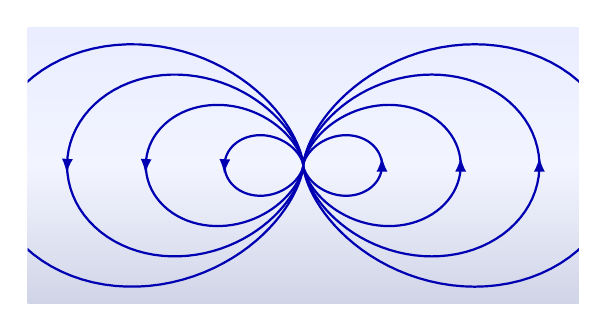
\begin{tikzpicture}
  \def\W{7.0}   % total length
  \def\H{3.5}   % total height
  \def\R{1.0}   % total distance
  \def\N{5}     % number of layers
  \def\t{\H/\N} % layer thickness
  % \draw[water,shading angle=0,draw=none]
    % (-0.52*\W,-0.52*\H) rectangle (0.52*\W,0.52*\H);
  % \draw[metal]
    % (0,0) circle(\R);

      % Clip to desired aspect ratio
  \clip (-0.5*\W,-0.5*\H) rectangle (0.5*\W,0.5*\H);
  
  % draw exact field lines for a dipole flow
  % use the expression r = K cos^2 theta of vector field lines of a dipole
  % use polar coordinates and foreach values of K
    \draw[water,shading angle=0,draw=none]
    (-0.52*\W,-0.52*\H) rectangle (0.52*\W,0.52*\H);
    
  \foreach \K in {1.0,2.0,3.0,4.0} {
    \draw[myblue,thick,postaction={decorate},decoration={markings,
      mark=at position {0.5} with {\arrow[xshift=3pt]{latex}},mark=at position {1} with {\arrow[xshift=3pt]{latex}}}]
      plot[domain=-3.14:3.14,samples=200] ({\K*cos(\x r)^2*cos(\x r)},{\K*cos(\x r)^2*sin(\x r)});
    % \draw[myblue,thick,postaction={decorate},decoration={markings,
    %   mark=at position {0.5} with {\arrow{latex}},mark=at position {0.69} with {\arrow{latex}}}]
    %   plot[domain=3.14:6.28,samples=200] ({\K*cos(\x r)^2*cos(\x r)},{\K*cos(\x r)^2*sin(\x r)});
  }
\end{tikzpicture}



\end{document}
